% !TeX root = ../main.tex
\problema{1}{Decaimiento sin fuente: tres esquemas de un paso}{6}

\begin{enunciado}
	Sea $\dfrac{\dd N}{\dd t} = -\lambda N$, $N(0) = N_0 = 100$, con $\lambda = \tfrac12$ y $h = \tfrac12$.
	\begin{enumerate}[label=(\alph*)]
		\item Deduzca los esquemas de Euler explícito, Euler implícito y Crank--Nicolson (CN)
		usando diferencias divididas de primer orden y el promedio de $f$ en $t_n$ y $t_{n+1}$.
		\item Calcule $N_1 \approx N(h)$ con cada esquema y el error absoluto respecto a la solución exacta.
		\item Obtenga el factor de amplificación $R(z)$, con $z = -\lambda h$, de cada esquema y
		determine su región de estabilidad. ¿Qué ocurre con $R$ cuando $\lambda h \to \infty$?
	\end{enumerate}
\end{enunciado}

\subsubsection*{Solución}
\[
\ddt{N} = -\lambda\,N(t), \qquad N(0) 	= N_0,
\]
Solución exacta es:
\[
\frac{\dd N}{\dd t} = -\lambda N
\;\Longrightarrow\; N(t) = N_0\,e^{-\lambda t} = 100\,e^{-t/2}
\]

\inciso{a}{Deduccion de los tres esquemas}


\paso{1}{Generación del mallado}
Se discretiza el tiempo con paso $h$:
\[
t_n = n h, \qquad n = 0, 1, 2, \dots, \qquad N_n \approx N(t_n).
\]

\textbf{Esquema 1: Euler explícito (diferencia dividida progresiva)}

\paso{2}{Colocación de la EDO en $t = t_n$}
\[
\left.\ddt{N}\right|_{t_n} = -\lambda\,N(t_n).
\]

\paso{3}{Sustituir la derivada por la diferencia progresiva}
Taylor alrededor de $t_n$:
\[
N(t_n + h) = N(t_n) + h\,N'(t_n) + \frac{h^2}{2!}\,N''(t_n) + \Order{h^3}.
\]
Despejando $N'(t_n)$:
\[
N'(t_n) = \frac{N(t_n + h) - N(t_n)}{h} - \frac{h}{2}\,N''(t_n) + \Order{h^2}.
\]
El término ($-\frac{h}{2}\,N''(t_n) + \Order{h^2}$) es el error de truncamiento de la diferencia
dividida, y es de orden $\Order{h}$. Sustituyendo en la EDO:
\[
\frac{N(t_{n+1}) - N(t_n)}{h} - \frac{h}{2}\,N''(t_n) + \Order{h^2} = -\lambda\,N(t_n).
\]
Quitamos el error de truncamiento y llamamos $N_n$ a la aproximación de $N(t_n)$:
\[
\frac{N_{n+1} - N_n}{h} = -\lambda\,N_n
\;\Longrightarrow\;
N_{n+1} - N_n = -\lambda h\,N_n .
\]

\resultado{N_{n+1} = (1 - \lambda h)\,N_n, \qquad n = 0, 1, 2, \dots}

Es explicito $N_{n+1}$ porque lo calculamos con $N_n$.

Es importante resaltar que $N(t_n) \neq N_n$. Al quitar el $\Order{h}$ ya no es el valor exacto en el nodo ya es una aproximación $N(t_n) \approx N_n$. Aqui lo que nos esta diciendo es que no se "quita" asi magicamente sino que se esta acumulando el error paso a pasao

\textbf{De forma general queda}
\begin{align*}
	N_1 &= (1 - \lambda h)\,N_0\\
	N_2 &= (1 - \lambda h)^2\,N_0\\
	&\;\;\vdots\\
	N_n &= (1 - \lambda h)^n\,N_0
\end{align*}


\textbf{Esquema 2: Euler implícito (diferencia dividida regresiva)}

\paso{2}{Colocación de la EDO en $t = t_n$}
\[
\left.\ddt{N}\right|_{t_n} = -\lambda\,N(t_n).
\]

\paso{3}{Sustituir la derivada por la diferencia regresiva}
Taylor alrededor de $t_n$, ahora hacia atrás:
\[
N(t_n - h) = N(t_n) - h\,N'(t_n) + \frac{h^2}{2!}\,N''(t_n) + \Order{h^3}.
\]
Despejando $N'(t_n)$:
\[
N'(t_n) = \frac{N(t_n) - N(t_n - h)}{h} + \frac{h}{2}\,N''(t_n) + \Order{h^2}.
\]
El error de truncamiento es $+\frac{h}{2}\,N''(t_n) + \Order{h^2}$, y nos damos cuenta que es de signo opuesto a la progresiva. Sustituyendo en la EDO y haciendo $N(t_n) \approx N_n$
\begin{align*}
	\frac{N_n - N_{n-1}}{h} &= -\lambda\,N_n\\
	N_n - N_{n-1} &= -\lambda h\,N_n\\
	N_n + \lambda h\,N_n &= N_{n-1}
	\;\Longrightarrow\; N_n\,(1 + \lambda h) = N_{n-1}
\end{align*}

\resultado{N_n = \frac{1}{1 + \lambda h}\,N_{n-1}, \qquad n = 1, 2, \dots}

\textbf{Caso general.}
\begin{align*}
	N_1 &= \frac{N_0}{1 + \lambda h}\\
	N_2 &= \frac{N_0}{(1 + \lambda h)^2}\\
	&\;\;\vdots\\
	N_n &= \frac{N_0}{(1 + \lambda h)^n}
\end{align*}

\paragraph{Esquema 3: Crank--Nicolson}

\paso{2}{Colocación de la EDO en $t_{\nmed}$}
$t_{\nmed} = t_n + h/2$:
\[
\left.\ddt{N}\right|_{t_{\nmed}} = -\lambda\,N(t_{\nmed}).
\]

Aquí la EDO no lo colocamos en un nodo entero ya que si lo hacemos daria
$\dfrac{N_{n+1} - N_{n-1}}{2h}$, con 2 incógnitas que no se conocen


%\paso{3}{Sustituir la derivada por la diferencia centrada}
%Se hacen dos desarrollos de Taylor alrededor de $t_{\nmed}$, con
%$t_{n+1} = t_{\nmed} + \tfrac{h}{2}$ y $t_n = t_{\nmed} - \tfrac{h}{2}$:
%\begin{align*}
%	N(t_{n+1}) &= N(t_{\nmed}) + \frac{h}{2}\,N'(t_{\nmed})
%	+ \frac{1}{2!}\left(\frac{h}{2}\right)^2 N''(t_{\nmed})
%	+ \frac{1}{3!}\left(\frac{h}{2}\right)^3 N'''(t_{\nmed}) + \Order{h^4}\\
%	N(t_n)     &= N(t_{\nmed}) - \frac{h}{2}\,N'(t_{\nmed})
%	+ \frac{1}{2!}\left(\frac{h}{2}\right)^2 N''(t_{\nmed})
%	- \frac{1}{3!}\left(\frac{h}{2}\right)^3 N'''(t_{\nmed}) + \Order{h^4}
%\end{align*}

\paso{3}{Sustituir la derivada por la diferencia centrada (paso $h/2$)}
Se hacen dos desarrollos de Taylor alrededor de $t_{\nmed}$, con
$t_{n+1} = t_{\nmed} + \tfrac{h}{2}$ y $t_n = t_{\nmed} - \tfrac{h}{2}$.
Tomare hasta $N^{(5)}$ para ver que terminos se van a cancelar y las derivadas estan evaluadas en $t_{\nmed}$
\begin{align*}
	N(t_{n+1}) &= N(t_{\nmed}) + \frac{h}{2}\,N'
	+ \frac{1}{2!}\left(\frac{h}{2}\right)^2 N''
	+ \frac{1}{3!}\left(\frac{h}{2}\right)^3 N'''
	+ \frac{1}{4!}\left(\frac{h}{2}\right)^4 N^{(4)}
	+ \frac{1}{5!}\left(\frac{h}{2}\right)^5 N^{(5)} + \Order{h^6}\\
	N(t_n)     &= N(t_{\nmed}) - \frac{h}{2}\,N'
	+ \frac{1}{2!}\left(\frac{h}{2}\right)^2 N''
	- \frac{1}{3!}\left(\frac{h}{2}\right)^3 N'''
	+ \frac{1}{4!}\left(\frac{h}{2}\right)^4 N^{(4)}
	- \frac{1}{5!}\left(\frac{h}{2}\right)^5 N^{(5)} + \Order{h^6}
\end{align*}

Restando las dos ecuacioneslos terminos pares se cancelan y los otros se duplican
\begin{align*}
	N(t_{n+1}) - N(t_n)
	&= \bigl[N(t_{\nmed}) - N(t_{\nmed})\bigr]
	+ \left[\frac{h}{2} + \frac{h}{2}\right] N'
	+ \Bigl[\cancel{\tfrac{1}{2!}\left(\tfrac{h}{2}\right)^2 N''} - \cancel{\tfrac{1}{2!}\left(\tfrac{h}{2}\right)^2 N''}\Bigr]\\
	&\quad + \frac{1}{3!}\left[\left(\frac{h}{2}\right)^3 + \left(\frac{h}{2}\right)^3\right] N'''
	+ \Bigl[\cancel{\tfrac{1}{4!}\left(\tfrac{h}{2}\right)^4 N^{(4)}} - \cancel{\tfrac{1}{4!}\left(\tfrac{h}{2}\right)^4 N^{(4)}}\Bigr]\\
	&\quad + \frac{1}{5!}\left[\left(\frac{h}{2}\right)^5 + \left(\frac{h}{2}\right)^5\right] N^{(5)} + \Order{h^6}
\end{align*}
entonces
\[
N(t_{n+1}) - N(t_n) = h\,N'(t_{\nmed}) + \frac{h^3}{24}\,N'''(t_{\nmed}) + \frac{h^5}{1920}\,N^{(5)}(t_{\nmed}) + \cdots
\]
\[
= h\,N'(t_{\nmed}) + \frac{h^3}{24}\,N'''(t_{\nmed}) + \Order{h^5}
\]

Despejando $N'(t_{\nmed})$
\begin{align*}
	h\,N'(t_{\nmed}) &= N(t_{n+1}) - N(t_n) - \frac{h^3}{24}\,N'''(t_{\nmed}) - \Order{h^5}\\
	N'(t_{\nmed}) &= \frac{N(t_{n+1}) - N(t_n)}{h} - \frac{h^2}{24}\,N'''(t_{\nmed}) + \Order{h^4}
\end{align*}

Sumando las ecuaciones
\begin{align*}
	N(t_{n+1}) + N(t_n)
	&= 2\,N(t_{\nmed})
	+ \Bigl[\cancel{\tfrac{h}{2}\,N'} - \cancel{\tfrac{h}{2}\,N'}\Bigr]
	+ \frac{2}{2!}\left(\frac{h}{2}\right)^2 N''\\
	&\quad + \Bigl[\cancel{\tfrac{1}{3!}\left(\tfrac{h}{2}\right)^3 N'''} - \cancel{\tfrac{1}{3!}\left(\tfrac{h}{2}\right)^3 N'''}\Bigr]
	+ \frac{2}{4!}\left(\frac{h}{2}\right)^4 N^{(4)} + \Order{h^6}
\end{align*}

\[
\frac{N(t_n) + N(t_{n+1})}{2} = N(t_{\nmed}) + \frac{h^2}{8}\,N''(t_{\nmed}) + \frac{h^4}{384}\,N^{(4)}(t_{\nmed}) + \cdots
= N(t_{\nmed}) + \frac{h^2}{8}\,N''(t_{\nmed}) + \Order{h^4}
\]
Despejando $N(t_{\nmed})$:
\[
N(t_{\nmed}) = \frac{N(t_n) + N(t_{n+1})}{2} - \frac{h^2}{8}\,N''(t_{\nmed}) + \Order{h^4}
\]

Los errores de truncamiento son entonces $\Order{h^2}$ 
\\
Sustituyendo en la EDO
$N'(t_{\nmed}) = -\lambda\,N(t_{\nmed})$
\[
\frac{N_{n+1} - N_n}{h} = -\lambda\,\frac{N_n + N_{n+1}}{2}.
\]

Algebra...
\begin{align*}
	2\left(N_{n+1} - N_n\right) &= -\lambda h\,N_n - \lambda h\,N_{n+1}\\
	2\,N_{n+1} + \lambda h\,N_{n+1} &= 2\,N_n - \lambda h\,N_n\\
	N_{n+1}\left(2 + \lambda h\right) &= N_n\left(2 - \lambda h\right)
\end{align*}

\resultado{N_{n+1} = \frac{2 - \lambda h}{2 + \lambda h}\,N_n
	= \frac{1 - \frac{\lambda h}{2}}{1 + \frac{\lambda h}{2}}\,N_n, \qquad n = 0, 1, 2, \dots}

su truncamiento es $\Order{h^2}$

\textbf{Caso general.}
\[
N_n = \left(\frac{2 - \lambda h}{2 + \lambda h}\right)^n N_0 .
\]

\begin{center}
	\begin{tabular}{lcccc}\toprule
		Esquema & Colocación & Diferencia & Formula & Truncamiento\\\midrule
		Euler explícito & $t_n$    & progresiva          & $N_{n+1} = (1 - \lambda h)\,N_n$                          & $\Order{h}$\\[2pt]
		Euler implícito & $t_n$    & regresiva           & $N_n = \dfrac{N_{n-1}}{1 + \lambda h}$                    & $\Order{h}$\\[6pt]
		Crank--Nicolson & $t_{\nmed}$ & centrada & $N_{n+1} = \dfrac{2 - \lambda h}{2 + \lambda h}\,N_n$      & $\Order{h^2}$\\\bottomrule
	\end{tabular}
\end{center}

\textbf{Error local y error global de los tres esquemas}


Forma común de los tres esquemas
Con $z = -\lambda h$ para los tres casos $N_{n+1} = R(z)\,N_n$
\begin{align*}
	\text{Euler explícito:}\quad & N_{n+1} = (1 - \lambda h)\,N_n = (1 + z)\,N_n, && R_{\mathrm{FE}}(z) = 1 + z\\
	\text{Euler implícito:}\quad & N_{n+1} = \frac{N_n}{1 + \lambda h} = \frac{N_n}{1 - z}, && R_{\mathrm{BE}}(z) = \frac{1}{1 - z}\\
	\text{Crank--Nicolson:}\quad & N_{n+1} = \frac{2 - \lambda h}{2 + \lambda h}\,N_n = \frac{2 + z}{2 - z}\,N_n, && R_{\mathrm{CN}}(z) = \frac{2 + z}{2 - z}
\end{align*}
La solución exacta es $N(t)=N_0\,e^{-\lambda t}$. Evaluada en $t_{n+1}=t_n+h$:
\begin{align*}
	N(t_{n+1}) &= N_0\,e^{-\lambda (t_n+h)}\\
	&= e^{-\lambda h}\,N_0\,e^{-\lambda t_n}\\
	&= e^{-\lambda h}\,N(t_n)
	= e^{z}\,N(t_n),
\end{align*}
es decir,
\begin{equation}\label{eq:p01_paso}
	N(t_{n+1}) = e^{z}\,N(t_n), \qquad z=-\lambda h .
\end{equation}
$R(z)$ debe parecerse a $e^{z}$ y su parecido mide el error de un paso

Definiciones
\begin{itemize}
	\item Error de truncamiento: error de la fórmula con que se aproxima la derivada
	\item Error local: error cometido en un solo paso suponiendo exacta la solución en el instante anterior,
	\item Error global: error acumulado en un tiempo final fijo $T$, con $n = T/h$ pasos
\end{itemize}

\inciso{b}{\texorpdfstring{Cálculo de $N_1$ y error absoluto}{Cálculo de N1 y error absoluto}}

Con $\lambda = \tfrac12$ y $h = \tfrac12$:
\[
\lambda h = \frac12\cdot\frac12 = \frac14, \qquad t_1 = 1\cdot h = \frac12 
\]

\textbf{Solución exacta:}
\[
N(h) = N_0\,e^{-\lambda h} = 100\,e^{-1/4} \approx 77.880078 
\]

\textbf{Euler explícito} ($n = 0$): $N_1 = (1 - \lambda h)\,N_0$
\[
N_1 = \left(1 - \tfrac14\right)(100) = \tfrac34(100) = 75 
\]

\textbf{Euler implícito} ($n = 1$): $N_1 = \dfrac{N_0}{1 + \lambda h}$
\[
N_1 = \frac{100}{1 + \frac14} = \frac{100}{5/4} = 80
\]

\textbf{Crank--Nicolson} ($n = 0$): $N_1 = \dfrac{2 - \lambda h}{2 + \lambda h}\,N_0$
\[
N_1 = \frac{2 - \frac14}{2 + \frac14}\,(100) = \frac{7/4}{9/4}\,(100) = \frac{7}{9}\,(100) = \frac{700}{9} \approx 77.777778
\]

Error absoluto $|N(h) - N_1|$
\begin{align*}
	\text{Euler explícito:}\quad & |100\,e^{-1/4} - 75| \approx 2.880078\\
	\text{Euler implícito:}\quad & |100\,e^{-1/4} - 80| \approx 2.119922\\
	\text{Crank--Nicolson:}\quad & \left|100\,e^{-1/4} - \tfrac{700}{9}\right| \approx 0.102301
\end{align*}

Comparación:
\begin{center}
	\begin{tabular}{lccc}\toprule
		Esquema & $N_1$ & exacta & $|N(h) - N_1|$\\\midrule
		Euler explícito & 75 & 77.880078 & 2.880078\\
		Euler implícito & 80 & 77.880078 & 2.119922\\
		Crank--Nicolson & $77.777778$ & 77.880078 & 0.102301\\\bottomrule
	\end{tabular}
\end{center}

Euler explícito subestima y Euler implícito sobreestima esto porque tienen el mismo orden de error a diferencia de Crank--Nicolson tiene un error menor.

\inciso{c}{\texorpdfstring{Factor de amplificación $R(z)$ y estabilidad}{Factor de amplificación R(z) y estabilidad}}

Los tres esquemas tienen la forma
\[
N_{n+1} = R(z)\,N_n \;\Longrightarrow\; N_n = R(z)^n\,N_0, \qquad z = -\lambda h .
\]
La solución exacta cumple
\[
N(t_{n+1}) = N_0\,e^{-\lambda (t_n + h)} = e^{-\lambda h}\,N(t_n) = e^{z}\,N(t_n),
\]
así que $R(z)$ es la aproximación de cada esquema a $e^{z}$.

\textbf{Obtención de $R(z)$.} Se usan las fórmulas del inciso (a) y $\lambda h = -z$:
\begin{align*}
	\text{Euler explícito:}\quad & N_{n+1} = (1 - \lambda h)\,N_n = (1 + z)\,N_n \;\Longrightarrow\; R_{\mathrm{FE}}(z) = 1 + z,\\
	\text{Euler implícito:}\quad & N_{n+1} = \frac{N_n}{1 + \lambda h} = \frac{N_n}{1 - z} \;\Longrightarrow\; R_{\mathrm{BE}}(z) = \frac{1}{1 - z},\\
	\text{Crank--Nicolson:}\quad & N_{n+1} = \frac{2 - \lambda h}{2 + \lambda h}\,N_n = \frac{2 + z}{2 - z}\,N_n \;\Longrightarrow\; R_{\mathrm{CN}}(z) = \frac{2 + z}{2 - z} = \frac{1 + z/2}{1 - z/2} .
\end{align*}

\textbf{Estabilidad absoluta.} Como $N_n = R^n N_0$, si $|R| > 1$ entonces $|N_n|$ crece sin límite
al avanzar en el tiempo, aunque la solución exacta decae. Si $|R| \le 1$ no crece. Por eso el esquema es
\textbf{estable} si
\[
|R(z)| \le 1 ,
\]
y la región de estabilidad es el conjunto de valores $z$ que cumplen esa desigualdad

\textbf{Con los datos del problema} ($\lambda h = \tfrac14$, $z = -\tfrac14$):
\[
R_{\mathrm{FE}} = 1 - \frac14 = \frac34, \qquad
R_{\mathrm{BE}} = \frac{1}{1 + \frac14} = \frac45, \qquad
R_{\mathrm{CN}} = \frac{2 - \frac14}{2 + \frac14} = \frac79 \approx 0.777778, \qquad
e^{-1/4} \approx 0.778801 .
\]
Los tres cumplen $|R| < 1$ y están dentro de su región de estabilidad

\textbf{Comportamiento cuando $\lambda h \to \infty$} ($z \to -\infty$, donde $e^{z} \to 0$).

\textbf{Euler explícito.}
\begin{align*}
	\lim_{\lambda h \to \infty} R_{\mathrm{FE}} &= \lim_{\lambda h \to \infty} \left(1 - \lambda h\right) = -\infty
\end{align*}

\textbf{Euler implícito.}
\begin{align*}
	\lim_{\lambda h \to \infty} R_{\mathrm{BE}} &= \lim_{\lambda h \to \infty} \frac{1}{1 + \lambda h} = 0
\end{align*}

\textbf{Crank--Nicolson.} Dividimos numerador y denominador entre $\lambda h$:
\begin{align*}
	\lim_{\lambda h \to \infty} R_{\mathrm{CN}}
	&= \lim_{\lambda h \to \infty} \frac{2 - \lambda h}{2 + \lambda h}\\
	&= \lim_{\lambda h \to \infty} \frac{\frac{2}{\lambda h} - 1}{\frac{2}{\lambda h} + 1}\\
	&= \frac{0 - 1}{0 + 1}\\
	&= -1
\end{align*}
\begin{center}
	\begin{tabular}{lccp{7cm}}\toprule
		Esquema & $\displaystyle\lim_{z \to -\infty} R(z)$ & Comportamiento\\\midrule
		Euler explícito & $-\infty$ & inestable: $|R|>1$, $|N_n|$ crece oscilando\\
		Euler implícito & $0$       & estable pero va a cero rapido\\
		Crank--Nicolson & $-1$      & estable ($|R|<1$) pero oscila \\\bottomrule
	\end{tabular}
\end{center}

Tabule los resultados en excel para diferentes valores de $\lambda h$ 
\begin{center}
	\begin{tabular}{cccccc}\toprule
		$\lambda h$ & $h$ & $R_{\mathrm{FE}}$ & $R_{\mathrm{BE}}$ & $R_{\mathrm{CN}}$ & $e^{-\lambda h}$\\\midrule
		$\tfrac14$ & $\tfrac12$ & $\tfrac34$ & $\tfrac45$ & $\tfrac79 \approx 0.777778$ & $0.778801$\\
		$1$ & $2$ & $0$ & $\tfrac12$ & $\tfrac13 \approx 0.333333$ & $0.367879$\\
		$2$ & $4$ & $-1$ & $\tfrac13 \approx 0.333333$ & $0$ & $0.135335$\\
		$3$ & $6$ & $-2$ & $\tfrac14$ & $-\tfrac15 = -0.2$ & $0.049787$\\
		$4$ & $8$ & $-3$ & $\tfrac15 = 0.2$ & $-\tfrac13 \approx -0.333333$ & $0.018316$\\
		$5$ & $10$ & $-4$ & $\tfrac16 \approx 0.166667$ & $-\tfrac37 \approx -0.428571$ & $0.006738$\\
		$10$ & $20$ & $-9$ & $\tfrac1{11} \approx 0.090909$ & $-\tfrac23 \approx -0.666667$ & $4.54\times10^{-5}$\\\bottomrule
	\end{tabular}
\end{center}

\textbf{Interpretación física.} Jugando con el programa de Python pude notar que todo depende del valor de $\lambda h$, a lo que me refiero es que tan grande es el paso $h$ comparado con la vida del isótopo $\lambda$.
Por ejemplo para pasos chicos los tres métodos siguen bien a la exacta pero conviene mas Crank--Nicolson.


Con pasos grandes ($\lambda h > 2$, aquí $h > 4$), Euler explícito ya no sirve porque la población se dispara oscilando, lo cual ya no tiene un sentido fisico. Y aca conviene Euler implícito que manda la población a cero como pasa en la realidad y CN no se aloca, pero tiene oscilación 

Para concluir para pasos chicos conviene  CN y para pasos grandes es decir isótopos de vida muy corta conviene Euler implícito.

\begin{figure}[htbp]
    \centering
    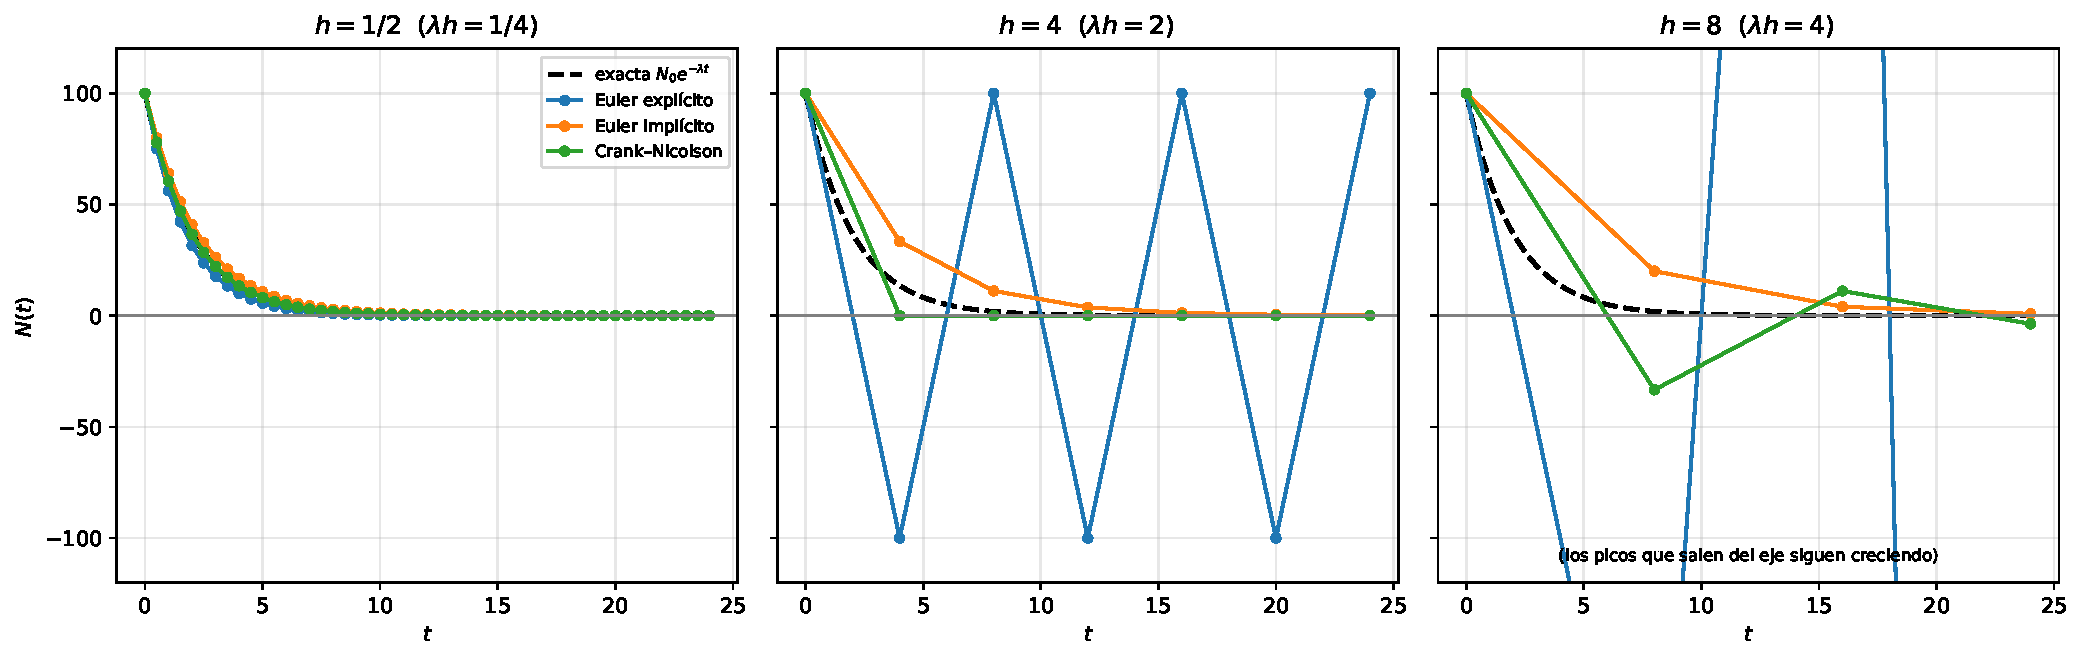
\includegraphics[width=\textwidth]{p1_decaimiento.pdf}
    \caption{Decaimiento real $N(t)$ contra $t$ ($\lambda=\tfrac12$, $N_0=100$)}
\end{figure}

\begin{figure}[htbp]
    \centering
    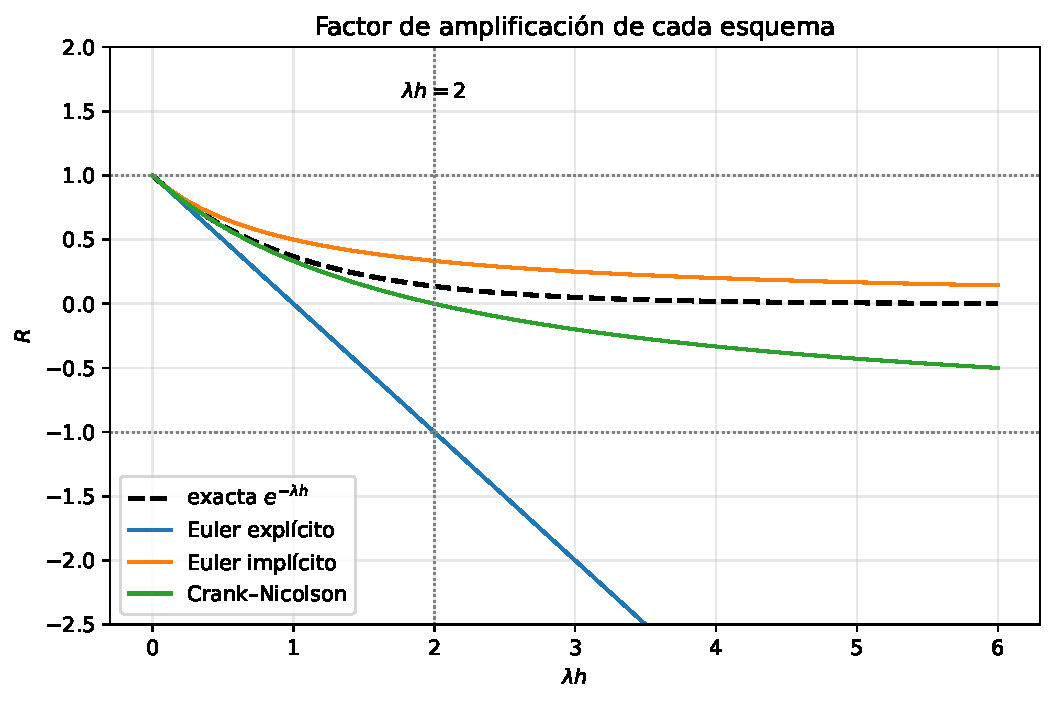
\includegraphics[width=0.8\textwidth]{p1_R_vs_lh.pdf}
    \caption{$R$ contra $\lambda h$}
\end{figure}

\begin{figure}[htbp]
    \centering
    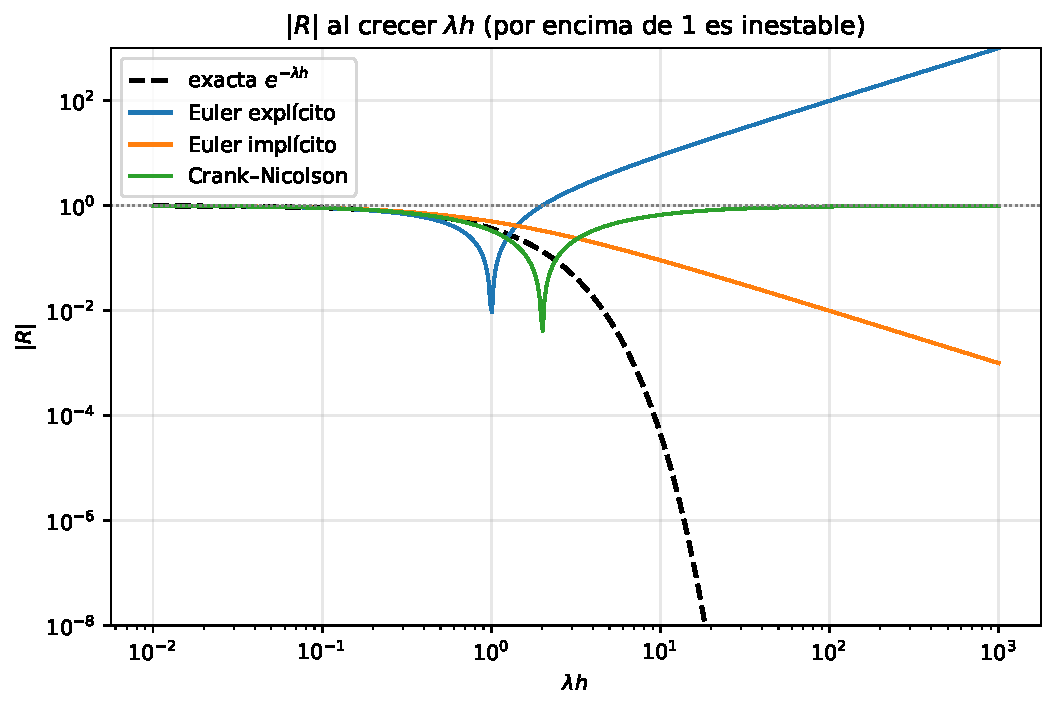
\includegraphics[width=0.8\textwidth]{p1_R_limite.pdf}
    \caption{$|R|$ cuando $\lambda h \to \infty$ (escala logarítmica).}
\end{figure}

Cree un notebook de Python para estudiar el comportamiento el repositorio lo subi a GitHub:
\url{\repoCIN}.
